\documentclass[12pt]{article}
 
\usepackage[margin=1in]{geometry}
\usepackage{amsmath,amsthm,amssymb, mathtools}
\usepackage[T1]{fontenc}
\usepackage{lmodern}
\usepackage{fixltx2e}
\usepackage[shortlabels]{enumitem}
\usepackage{mathrsfs}
\usepackage{kbordermatrix}

\usepackage{graphicx}
\usepackage{bbm}

\renewcommand{\kbldelim}{(}% Left delimiter
\renewcommand{\kbrdelim}{)}% Right delimiter
 
\newcommand{\N}{\mathbb{N}}
\newcommand{\R}{\mathbb{R}}
\newcommand{\Z}{\mathbb{Z}}
\newcommand{\Q}{\mathbb{Q}}
 
\newenvironment{theorem}[2][Theorem]{\begin{trivlist}
\item[\hskip \labelsep {\bfseries #1}\hskip \labelsep {\bfseries #2.}]}{\end{trivlist}}
\newenvironment{lemma}[2][Lemma]{\begin{trivlist}
\item[\hskip \labelsep {\bfseries #1}\hskip \labelsep {\bfseries #2.}]}{\end{trivlist}}
\newenvironment{exercise}[2][Exercise]{\begin{trivlist}
\item[\hskip \labelsep {\bfseries #1}\hskip \labelsep {\bfseries #2.}]}{\end{trivlist}}
\newenvironment{problem}[2][Problem]{\begin{trivlist}
\item[\hskip \labelsep {\bfseries #1}\hskip \labelsep {\bfseries #2.}]}{\end{trivlist}}
\newenvironment{question}[2][Question]{\begin{trivlist}
\item[\hskip \labelsep {\bfseries #1}\hskip \labelsep {\bfseries #2.}]}{\end{trivlist}}
\newenvironment{corollary}[2][Corollary]{\begin{trivlist}
\item[\hskip \labelsep {\bfseries #1}\hskip \labelsep {\bfseries #2.}]}{\end{trivlist}}
\newcommand{\textfrac}[2]{\dfrac{\text{#1}}{\text{#2}}}
\newcommand{\floor}[1]{\left\lfloor #1 \right\rfloor}

\newenvironment{amatrix}[1]{%
  \left(\begin{array}{@{}*{#1}{c}|c@{}}
}{%
  \end{array}\right)
}

\DeclareMathOperator*{\E}{\mathbb{E}}


\begin{document}

\title{Stochastic Processes: Midterm Exam}

\author{Chris Hayduk}
\date{October 21, 2020}

\maketitle

\begin{problem}{1}
\end{problem}

\begin{enumerate}[label=(\Alph*)]

\item We know the deck contains 10 cards and that the draws are independent and uniform. Hence, the probability of drawing any single card is $\frac{1}{10}$. So, if we suppose that we have seen a certain card $i$ times in a row, the probability of selecting that card for the $i+1$ time in a row would be $\frac{1}{10}$. Thus, it is clear that, for $i \geq 1$, we have $P(X_{n+1} = i + 1 | X_{n} = i, X_{n-1} = i_{n_1}, \cdots X_0 = 0) = \frac{1}{10} = P(X_{n+1} = i + 1 | X_{n} = i)$.\\

In the case of $n = 0$, we have $X_0 = 0$ by definition. In addition, note that $P(X_{n+1} = 0 | X_{n} = i) = \frac{9}{10}$ for $i \neq 0$. Since $X_{n+1} = i + 1, X_{n+1} = 0$ are the only possible transitions from $X_n = i, i \neq 0$, we have that they add up to $1$ as required. Moreover, we can define any other transitions as $0$ probability, so $p(i, j) \geq 0$ for any $i, j$ in the state space as required. In the case of $i = 0$, these conditions still hold, as the only possible transition is $P(X_{n+1} = 1 | X_n = 0) = 1$ since we must choose a card.\\

As a result, we have that this defines a valid Markov chain with the following transition probability matrix,
\begin{align*}
p = \kbordermatrix{
    & 0 & 1 & 2 & 3 & 4 & \cdots \\
    0 & 0 & 1 & 0 & 0 & 0 & \cdots\\
    1 & 9/10 & 0 & 1/10 & 0 & 0 & \cdots\\
    2 & 9/10 & 0 & 0 & 1/10 & 0 & \cdots\\
    3 & 9/10 & 0 & 0 & 0 & 1/10 & \cdots\\
    \vdots & & & \vdots & & & \cdots
  }
\end{align*}

That is, we have,
\begin{align*}
p(0, 1) &= 1
\end{align*}

and for $i > 0$, we have,
\begin{align*}
p(i, 0) &= 9/10\\
p(i, i+1) &= 1/10
\end{align*}

\item Let us consider the transition matrix $\tilde{p}$, where we eliminate every state after $9$ and consider state $9$ an absorbing state:

\begin{align*}
\tilde{p} = \kbordermatrix{
    & 0 & 1 & 2 & 3 & 4 & 5 & 6 & 7 & 8 & 9\\
    0 & 0 & 1 & 0 & 0 & 0 & 0 & 0 & 0 & 0 & 0\\
    1 & 9/10 & 0 & 1/10 & 0 & 0 & 0 & 0 & 0 & 0 & 0\\
    2 & 9/10 & 0 & 0 & 1/10 & 0 & 0 & 0 & 0 & 0 & 0\\
    3 & 9/10 & 0 & 0 & 0 & 1/10 & 0 & 0 & 0 & 0 & 0\\
    4 & 9/10 & 0 & 0 & 0 & 0 & 1/10 & 0 & 0 & 0 & 0\\
    5 & 9/10 & 0 & 0 & 0 & 0 & 0 & 1/10 & 0 & 0 & 0\\
    6 & 9/10 & 0 & 0 & 0 & 0 & 0 & 0 & 1/10 & 0 & 0\\
    7 & 9/10 & 0 & 0 & 0 & 0 & 0 & 0 & 0 & 1/10 & 0\\
    8 & 9/10 & 0 & 0 & 0 & 0 & 0 & 0 & 0 & 0 & 1/10\\
    9 & 0 & 0 & 0 & 0 & 0 & 0 & 0 & 0 & 0 & 1
  }
\end{align*}

We are able to make this change because we have not altered any of the states which lead to $9$ and for the purposes of this analysis, we do not need to consider any of the states which come after $9$. Let us now construct the matrix $r$ by removing the rows and columns corresponding to state $9$:
\begin{align*}
r = \kbordermatrix{
    & 0 & 1 & 2 & 3 & 4 & 5 & 6 & 7 & 8\\
    0 & 0 & 1 & 0 & 0 & 0 & 0 & 0 & 0 & 0\\
    1 & 9/10 & 0 & 1/10 & 0 & 0 & 0 & 0 & 0 & 0\\
    2 & 9/10 & 0 & 0 & 1/10 & 0 & 0 & 0 & 0 & 0\\
    3 & 9/10 & 0 & 0 & 0 & 1/10 & 0 & 0 & 0 & 0\\
    4 & 9/10 & 0 & 0 & 0 & 0 & 1/10 & 0 & 0 & 0\\
    5 & 9/10 & 0 & 0 & 0 & 0 & 0 & 1/10 & 0 & 0\\
    6 & 9/10 & 0 & 0 & 0 & 0 & 0 & 0 & 1/10 & 0\\
    7 & 9/10 & 0 & 0 & 0 & 0 & 0 & 0 & 0 & 1/10\\
    8 & 9/10 & 0 & 0 & 0 & 0 & 0 & 0 & 0 & 0  }
\end{align*}

Now we must evaluate $I - r$, where $I$ is the $9 \times 9$ identity matrix,
\begin{align*}
I - r = \kbordermatrix{
    & 0 & 1 & 2 & 3 & 4 & 5 & 6 & 7 & 8\\
    0 & 1 & -1 & 0 & 0 & 0 & 0 & 0 & 0 & 0\\
    1 & -9/10 & 1 & -1/10 & 0 & 0 & 0 & 0 & 0 & 0\\
    2 & -9/10 & 0 & 1 & -1/10 & 0 & 0 & 0 & 0 & 0\\
    3 & -9/10 & 0 & 0 & 1 & -1/10 & 0 & 0 & 0 & 0\\
    4 & -9/10 & 0 & 0 & 0 & 1 & -1/10 & 0 & 0 & 0\\
    5 & -9/10 & 0 & 0 & 0 & 0 & 1 & -1/10 & 0 & 0\\
    6 & -9/10 & 0 & 0 & 0 & 0 & 0 & 1 & -1/10 & 0\\
    7 & -9/10 & 0 & 0 & 0 & 0 & 0 & 0 & 1 & -1/10\\
    8 & -9/10 & 0 & 0 & 0 & 0 & 0 & 0 & 0 & 1  }
\end{align*}

Once we take the inverse and multiply by the column vector of all $1$s, we get,
\begin{align*}
(I - r)^{-1} \mathbbm{1} &= \begin{pmatrix}
211,111,110\\
\vdots
\end{pmatrix}
\end{align*}

So the expected number of moves starting from state $0$ is $211,111,110$. For a brief sanity check, we see that the probability of seeing a specific card 9 times in a row is 
\begin{align*}
1 \cdot \frac{1}{10^8} &= \frac{1}{100,000,000}\\
&= 1 \times 10^{-8}
\end{align*}

So our answer makes sense given the extremely low probability of seeing $9$ identical cards in a row.
\end{enumerate}

\begin{problem}{2}
\end{problem}

Let us first examine $f_n(d)$. After computing the recursion for the first few values of $n$, we get,
\begin{align*}
f_0(d) &= 0\\
f_1(d) &= \frac{f_0(c) + f_0(e)}{2} = 0\\
f_2(d) &= \frac{f_0(a) + f_0(b) +f_0(d) + f_0(d)}{4} = \frac{f_0(a) + f_0(b)}{4} = \frac{1}{4}\\
f_3(d) &= \frac{f_0(a) + f_0(b) + 3f_0(c) + 3f_0(e)}{8} = \frac{f_0(a) + f_0(b)}{8} = \frac{1}{8}\\
f_4(d) &= \frac{4f_0(a) + 4f_0(b) + f_0(c) + 6f_0(d) + f_0(e)}{16} = \frac{4f_0(a) + 4f_0(b)}{16} = \frac{4}{16}\\
f_5(d) &= \frac{5f_0(a) + 5f_0(b) + 10f_0(c) + 2f_0(d) + 10f_0(e)}{32} = \frac{5f_0(a) + 5f_0(b)}{32} = \frac{5}{32}\\
f_6(d) &= \frac{15f_0(a) + 15f_0(b) + 7f_0(c) + 20f_0(d) + 7f_0(e)}{64} = \frac{15f_0(a) + 15f_0(b)}{64} = \frac{15}{64}\\
f_7(d) &= \frac{22f_0(a) + 22f_0(b) + 35f_0(c) + 14f_0(d) + 35f_0(e)}{128} = \frac{22f_0(a) + 22f_0(b)}{128} = \frac{22}{128}\\
&\vdots
\end{align*}

I believe this is converging to $\frac{f_0(a) + f_0(b) + f_0(c) + f_0(d) + f_0(e)}{5} = 0.2$ (ie. the average value of the original pentagon vertices), with the even terms converging from above and the odd terms converging from below. I claim that $f_n$ converges to this value for any $x \in \{a, b, c, d, e\}$.\\

Observe that the denominator is $2^n$ and there are $2^n$ terms of $f_0$ in the numerator for all $n \geq 1$. I claim that the proportion of terms in the numerator which belong to the non-zero $f_0$ values (ie. $f_0(a)$ and $f_0(b)$) approaches $\frac{2^n}{5}$. That is, the function approaches $\frac{(2^n/5) \cdot (f_0(a) + f_0(b))}{2^n}$

\newpage
\begin{problem}{3}
\end{problem}

Let us label the vertices as follows:

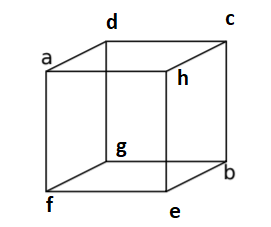
\includegraphics{cube.png}

Since each vertex is connected to three other vertices, we have that the transition probability is $1/3$ between any two vertices sharing an edge and $0$ between all others. This yields the following transition probability matrix:
\begin{align*}
p &= \kbordermatrix{
    & a & b & c & d & e & f & g & h\\
    a & 0 & 0 & 0 & 1/3 & 0 & 1/3 & 0 & 1/3\\
    b & 0 & 0 & 1/3 & 0 & 1/3 & 0 & 1/3 & 0\\
    c & 0 & 1/3 & 0 & 1/3 & 0 & 0 & 0 & 1/3\\
    d & 1/3 & 0 & 1/3 & 0 & 0 & 0 & 1/3 & 0\\
    e & 0 & 1/3 & 0 & 0 & 0 & 1/3 & 0 & 1/3\\
    f & 1/3 & 0 & 0 & 0 & 1/3 & 0 & 1/3 & 0\\
    g & 0 & 1/3 & 0 & 1/3 & 0 & 1/3 & 0 & 0\\
    h & 1/3 & 0 & 1/3 & 0 & 1/3 & 0 & 0 & 0
    }
\end{align*}

Now we need to find $P(T_a < T_b | X_0 = a)$. That is, the probability that the first return to $a$ will be sooner than the first return to $b$ when we start from state $a$.\\

We have three distinct cases here: $X_1 = d$, $X_1 = h$, and $X_1 = f$. We will consider all three cases with both $a$ and $b$ as absorbing states. Thus, the probability $P(T_a < T_b | X_0 = a)$ will be equivalent to $\frac{1}{3} (\lim_{n \to \infty} \tilde{p}^n(d, a) + \lim_{n \to \infty} \tilde{p}^n(h, a) + \lim_{n \to \infty} \tilde{p}^n(f, a))$. This is true because, since $a$ and $b$ are both absorbing states, $\lim_{n \to \infty} \tilde{p}^n(d, a)$ will show the probability of reaching $a$ (and therefore not reaching $b$) starting from state $d$. The case of the other two states is the same. We multiply by $1/3$ because each possibility for $X_1 = d, h, f$ has a $1/3$ chance of occurring.\\

Let us now set up the new transition probability matrix:
\begin{align*}
\tilde{p} &= \kbordermatrix{
    & a & b & c & d & e & f & g & h\\
    a & 1 & 0 & 0 & 0 & 0 & 0 & 0 & 0\\
    b & 0 & 1 & 0 & 0 & 0 & 0 & 0 & 0\\
    c & 0 & 1/3 & 0 & 1/3 & 0 & 0 & 0 & 1/3\\
    d & 1/3 & 0 & 1/3 & 0 & 0 & 0 & 1/3 & 0\\
    e & 0 & 1/3 & 0 & 0 & 0 & 1/3 & 0 & 1/3\\
    f & 1/3 & 0 & 0 & 0 & 1/3 & 0 & 1/3 & 0\\
    g & 0 & 1/3 & 0 & 1/3 & 0 & 1/3 & 0 & 0\\
    h & 1/3 & 0 & 1/3 & 0 & 1/3 & 0 & 0 & 0
    }
\end{align*}

Note that we can reformulate our above discussion such that,
\begin{align*}
P(T_a < T_b | X_0 = a) &= \frac{1}{3} (\lim_{n \to \infty} \tilde{p}^n(d, a) + \lim_{n \to \infty} \tilde{p}^n(h, a) + \lim_{n \to \infty} \tilde{p}^n(f, a))\\
&= \frac{1}{3} (P(V_a < V_b | X_0 = d) + P(V_a < V_b | X_0 = h) + P(V_a < V_B | X_0 = f))
\end{align*}

This is possible since $a$ and $b$ are both absorbing states now.\\

Now let $P_x(V_a < V_b) =: j(x)$. Let $j(a) = 1$ and $j(b) = 0$. Then we have the following system of equations,
\begin{align*}
j(a) &= 1\\
j(b) &= 0\\
j(c) &= \frac{1}{3}(j(d) + j(h))\\
j(d) &= \frac{1}{3}(1 + j(c) + j(g))\\
j(e) &= \frac{1}{3}(j(f) + j(h))\\
j(f) &= \frac{1}{3}(1 + j(e) + j(g))\\
j(g) &= \frac{1}{3}(j(d) + j(f))\\
j(h) &= \frac{1}{3}(1 + j(c) + j(e))
\end{align*}

Note also that we must have $j(d) = j(h) = j(f)$ and $j(g) = j(e) = j(c)$ because each of these vertices are the same number of moves away from $a$ and $b$ and each move has the same probability. In addition, each vertex that they can possibly move to is the same number of moves from $a$ or $b$. So let's revise this system of equations, using one representative from each equivalence class,
\begin{align*}
j(a) &= 1\\
j(b) &= 0\\
j(c) &= \frac{2j(d)}{3}\\
j(d) &= \frac{1}{3}(1 + 2j(g))\\
j(e) &= \frac{2j(d)}{3}\\
j(f) &= \frac{1}{3}(1 + 2j(g))\\
j(g) &= \frac{2j(d)}{3}\\
j(h) &= \frac{1}{3}(1 + 2j(g))
\end{align*}

Plugging $j(g)$ into the equation for $j(d)$ yields,
\begin{align*}
j(d) = \frac{3}{5}
\end{align*}

and
\begin{align*}
j(g) = \frac{2}{5}
\end{align*}

Hence, our system of equations is,
\begin{align*}
j(a) &= 1\\
j(b) &= 0\\
j(c) &= \frac{2}{5}\\
j(d) &= \frac{3}{5}\\
j(e) &=\frac{2}{5}\\
j(f) &= \frac{3}{5}\\
j(g) &= \frac{2}{5}\\
j(h) &= \frac{3}{5}
\end{align*}

Thus, we have,
\begin{align*}
P(T_a < T_b | X_0 = a) &= \frac{1}{3} (P(V_a < V_b | X_0 = d) + P(V_a < V_b | X_0 = h) + P(V_a < V_B | X_0 = f))\\
&= \frac{1}{3} (\frac{3}{5} + \frac{3}{5} + \frac{3}{5})\\
&= \frac{3}{5}
\end{align*}

For a quick sanity check, we compute the matrix powers of $\tilde{p}$ (done in the R programming language) and find,
\begin{align*}
\tilde{p}^{1000} &= \kbordermatrix{
    & a & b & c & d & e & f & g & h\\
    a & 1 & 0 & 0 & 0 & 0 & 0 & 0 & 0\\
    b & 0 & 1 & 0 & 0 & 0 & 0 & 0 & 0\\
    c & 0.4 & 0.6 & 0 & 0 & 0 & 0 & 0 & 0\\
    d & 0.6 & 0.4 & 0 & 0 & 0 & 0 & 0 & 0\\
    e & 0.4 & 0.6 & 0 & 0 & 0 & 0 & 0 & 0\\
    f & 0.6 & 0.4 & 0 & 0 & 0 & 0 & 0 & 0\\
    g & 0.4 & 0.6 & 0 & 0 & 0 & 0 & 0 & 0\\
    h & 0.6 & 0.4 & 0 & 0 & 0 & 0 & 0 & 0
    }
\end{align*}

Hence, we have $P(V_a < V_b | X_0 = d) = P(V_a < V_b | X_0 = h) = P(V_a < V_B | X_0 = f) = 0.6 = \frac{3}{5}$ as we have shown above.

\begin{problem}{4}
\end{problem}

Fix $i \in \mathcal{S}$. Suppose $X_n = i$ for some $n$. Now consider the state $j \in S$ such that $j < i$. It is possible to reach $j$ from $i$ because $p(i, 0) = 1/4$. Once we are at $0$, we have that $p(0, 1) = 3/4$, $p(1, 2) = 3/4$. Hence, by induction, we have $p(j-1, j) = 3/4$.\\

Now assume $j > i$. We can perform the same process, except without returning to $0$. We have $p(i, i+1) = p(i+1, i+2) = \cdots = p(j-1, j) = 3/4$. Thus, we can reach $j$ from $i$ when $j > i$.\\

Lastly, when $j = i$, we need to perform the same process as $j < i$. We can return to $0$ with probability $p(i, 0) = 1/4$, and then we have, $p(0, 1) = p(1, 2) = \cdots p(i-1, i) = 3/4$. Hence, we have that we can reach $i$ from state $i$.\\

Since $i$ was arbitrary and we covered every possible case for another state $j$, this holds for any state in $\mathcal{S}$. Thus, every state in $\mathcal{S}$ communicates with every other state, and so the chain is irreducible.\\

Now we need to show that there is a positive recurrent state in the chain. Let us consider state $0$. Consider $P_0(T_0 = \infty) = 1 - P_0(T_0 < \infty)$. We have that,
\begin{align*}
P_0(T_0 = \infty) &= p(0, 1) \cdot p(1, 2) \cdot p(2, 3) \cdot p(3, 4) \cdots\\
&= \sum_{i=0}^{\infty} p(i, i+1)
\end{align*}

Since $p(i, i+1) = 3/4$ for every $i \in \mathcal{S}$, this sum is equivalent to,
\begin{align*}
\lim_{n \to \infty} 3n/4
\end{align*}

Thus, we have that,
\begin{align*}
P_0(T_0 < \infty) &= 1 - P_0(T_0 = \infty)\\
&= 1 - \lim_{n \to \infty} 3n/4\\
&= 1 - 0 = 1
\end{align*}

Hence, $0$ is recurrent in the sense that we will certainly return. Now consider $E_0T_0$. Note that from each state $x$, we have probability $1/4$ of returning to $0$, and probability $3/4$ of continuing to state $x+1$. Hence, we can consider each state to be an independent trial where we have probability $1/4$ of reaching $0$ and probability $3/4$ of not reaching $0$. Thus we can model this problem as an unfair coin with $1/4$ chance of heads and $3/4$ chance of tails.\\

Hence, we can use the geometric distribution, which models the number of Bernoulli trials needed to get one success. The mean of this sequence is $1/p$ where $p$ is the probability of success. In our case, $p = 1/4$, so we have
\begin{align*}
\frac{1}{p} &= 4
\end{align*}

Since this is the mean number of trials before we reach $1$ success (ie. a return to state $0$), then we have that this is precisely $E_0T_0$. Hence, $E_0T_0 = 4 < \infty$. Hence $0$ is a positive recurrent state.\\

Now, since the chain is irreducible and $0$ is a positive recurrent state, by Theorem 1.30 in Durrett, we have that all states are positive recurrent. Thus, the chain is positive recurrent. In addition, Theorem 1.30 tells us that there exists a stationary distribution $\pi$. Hence, we need to find $\pi$ such that,
\begin{align*}
\pi p = \pi
\end{align*}

where $p$ is the transition probability matrix, which is given by,
\begin{align*}
p = \kbordermatrix{
    & 0 & 1 & 2 & 3 & 4 & \cdots \\
    0 & 1/4 & 3/4 & 0 & 0 & 0 & \cdots\\
    1 & 1/4 & 0 & 3/4 & 0 & 0 & \cdots\\
    2 & 1/4 & 0 & 0 & 3/4 & 0 & \cdots\\
    3 & 1/4 & 0 & 0 & 0 & 3/4 & \cdots\\
    \vdots & & & \vdots & & & \cdots
  }
\end{align*}

So, if we let $\pi$ be given by,
\begin{align*}
\pi = \begin{pmatrix}
\pi_0 & \pi_1 & \pi_2 & \pi_3 & \cdots
\end{pmatrix}
\end{align*}

Then we get that $\pi p = \pi$ implies,
\begin{align*}
\frac{1}{4} \sum_{i=0}^{\infty} \pi_i &= \pi_0\\
\frac{3}{4} \pi_0 &= \pi_1\\
\frac{3}{4} \pi_1 &= \pi_2\\
\frac{3}{4} \pi_2 &= \pi_3\\
&\vdots
\end{align*}

We can use the above equations to define $\pi_i$ with $i \geq 1$ in terms of $\pi_0$. We get,
\begin{align*}
\pi_i = \left(\frac{3}{4}\right)^i\pi_0
\end{align*}

Since $\pi$ defines a valid distribution, we also need $\sum_{i=0}^{\infty} \pi(i) = 1$. This yields,
\begin{align*}
&\sum_{i=0}^{\infty} \left(\frac{3}{4}\right)^i\pi_0 = 1\\
\implies &\pi_0 \sum_{i=0}^{\infty} \left(\frac{3}{4}\right)^i = 1
\end{align*}

We have that $\sum_{i=0}^{\infty} \left(\frac{3}{4}\right)^i$ converges to $4$, so this gives us,
\begin{align*}
&\pi_0 \sum_{i=0}^{\infty} \left(\frac{3}{4}\right)^i = 1\\
\implies &4\pi_0 = 1\\
\implies &\pi_0 = \frac{1}{4}
\end{align*}

Verifying this value in the equation for $\pi_0$ gives us,
\begin{align*}
&\frac{1}{4} \sum_{i=0}^{\infty} \left(\frac{3}{4}\right)^i\pi_0 = \pi_0\\
\implies &\frac{1}{4} \pi_0 \sum_{i=0}^{\infty} \left(\frac{3}{4}\right)^i = \pi_0\\
\implies &\frac{1}{4} \cdot \frac{1}{4} \cdot \sum_{i=0}^{\infty} \left(\frac{3}{4}\right)^i = \frac{1}{4}\\
\implies &\frac{1}{16} \cdot 4 = \frac{1}{4}\\
\implies &\frac{1}{4} = \frac{1}{4}
\end{align*}

as required. In addition, since $0 \leq \left(\frac{3}{4}\right)^i\pi_0 \leq 1/4$ for every $i \geq 0$, along with the fact that $\sum \pi_i = 1$, we have that $\pi$ defines a valid probability distribution.\\

Thus, we have that the stationary distribution is given by,
\begin{align*}
\pi_i &= \frac{1}{4} \cdot  \left(\frac{3}{4}\right)^i\\
&= \frac{3^i}{4^{i+1}}
\end{align*}

for all $i \geq 0$.

\end{document}